  Avant d'attaquer les spécificités des modèles simulés et les lois exactes associées, il est nécessaire de valider les méthodes numériques exposées dans le Chapitre \ref{ch-31} et d'en déterminer les biais. Dans la section \ref{sec-321}, les résultats de la loi exacte \cacro{IMHDH} seront comparés aux résultats de \cacro{F21}. %Dans la section \ref{sec-323}, les résultats \acs{MHD} avec pression isotrope dérivée dans le Chapitre \ref{ch-13} seront comparés aux prédictions de \ac{A18}. 
  Enfin, dans la section \ref{sec-323}, une méthode d'estimation de l'incertitude sur nos résultats sera proposée. 
  Les simulations utilisées dans ces études comparatives sont CGL1 et CGL3 (voir détail \tabref{tab:setups} et \tabref{tab:setups_hd}). Elles font partie des simulations du modèle \sacro{CGLHPe} analysées par \cacro{F21} et elles feront l'objet du Chapitre \ref{ch-33}.  

  
 
% Pour chaque simulation, une temps a été sélectionnée. À partir de cette temps, la simulation a été relancée sur quelques pas de temps rapprochés avec extraction des quantités pour chacun d'eux. Sauf exception de la  \figref{fig:compainc_t}, tous les résultats montrés dans ce chapitre correspondent à une moyenne de ces échantillons. Pour CGL1, la temps correspond au temps utilisé par F21, pour CGL3, c'est la temps précédente, \ac{F21} analysant le temps $t =\num{362}$ mais les lois exactes étant statistiquement stationnaire, on s'attend à retrouver des résultats similaires.    

 \section{Comparaison de résultats Inc-MHD-Hall avec pression isotrope et schémas numériques}
 \label{sec-321}
 
 \subsection{Comparaison avec des  résultats Inc-MHD-Hall}

 Afin de valider les méthodes et choix décrits dans le Chapitre \ref{ch-31}, nous avons calculé avec les données de CGL1 et CGL3 les quantités comparées par \cacro{F21} : 
 \begin{itemize}
     \item $\varepsilon_{MHD}$, provenant de la loi \cacro{PP98} (équation \eqref{eq:synth_inc_EL}),
     \item $\varepsilon_{Hall}$, la correction Hall incompressible (équation \eqref{eq:corr_hallinc}),
     \item $\varepsilon_{MHD-Hall} = \varepsilon_{MHD} + \varepsilon_{Hall}$, qui correspond au résultat de la loi \cacro{IMHDH} dérivée par \cite{ferrand_exact_2019}.
 \end{itemize} 
 Pour CGL1, le temps sélectionné, indiqué dans la \tabref{tab:setups}, est celui utilisée par \cacro{F21}. Ce n'est pas le cas pour CGL3, pour laquelle \cacro{F21} utilise $t =\num{357}$. Afin de ne pas apporter d'incertitude à notre comparaison en changeant les données utilisées, les résultats seront exceptionnellement donnés pour $t =\num{357}$ dans cette section. 
 
 Par conséquent, aucune différence que l'on pourra noter ne proviendra des données, des expressions des quantités ou de leur domaine de validité. Les différences entre les résultats résideront dans les schémas numériques utilisés. On a indiqué le nôtre par la mention \cacro{FEL} et celui de \cacro{F21} par \og F21\fg{}.  Nos résultats sont présentés sur la \figref{fig:compainc} par des lignes pleines et sont accompagnés de ceux des figures 3 et 5 de \cacro{F21} en pointillés. 
 
 \begin{figure}[!ht]
  \centering
 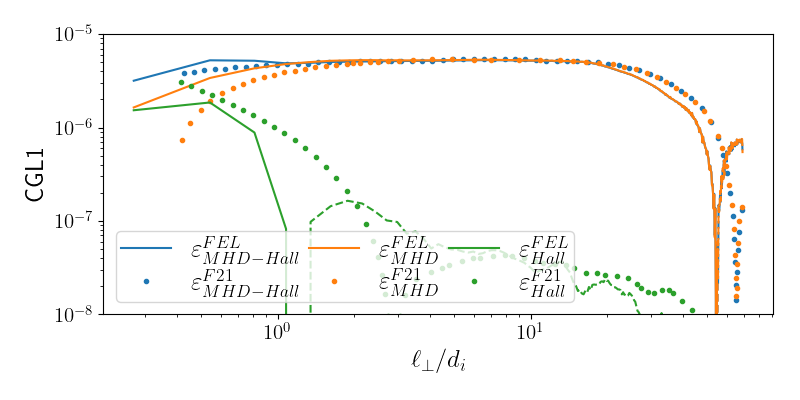
\includegraphics[width=0.85\linewidth,trim=0.5cm 0.5cm 0.5cm 0.5cm, clip=true]{./Mainmatter/Part_3/images_ch2/CGL1_compainc}
 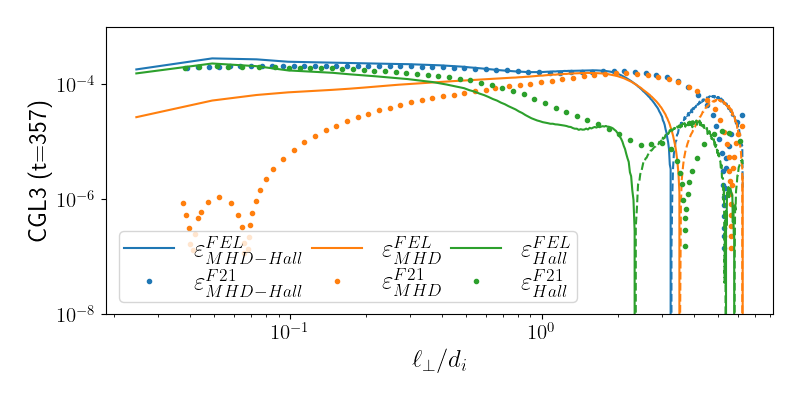
\includegraphics[width=0.85\linewidth,trim=0.5cm 0.5cm 0.5cm 0.5cm, clip=true]{./Mainmatter/Part_3/images_ch2/CGL3_compainc}
 \cprotect\caption{Mode de représentation : \cacro{1D} en fonction de \ensuremath{\ell_{\perp}} normalisé par \ensuremath{d_i}. Lignes pleines : nos résultats (avec en lignes discontinues les valeurs négatives). Pointillés : résultats extraits des figures 3 et 5 de \cacro{F21}. Bleu : \ensuremath{\varepsilon_{MHD-Hall}}. Orange : \ensuremath{\varepsilon_{MHD}}. Vert : \ensuremath{\varepsilon_{Hall}}. Haut : CGL1. Bas : CGL3 (\ensuremath{t =\num{357}}).}
 \label{fig:compainc}
 \end{figure}
 
 Tout d'abord, pour chaque simulation, on retrouve les points physiques attendus : 
 \begin{itemize}
     \item Pour CGL1 : une zone inertielle \cacro{MHD} telle que $\varepsilon_{MHD-Hall} = \varepsilon_{MHD}$ (resp. courbe bleue et orange) et une augmentation de $\varepsilon_{Hall}$ (courbe verte) en allant vers les petites échelles.
     \item Pour CGL3 : une croissance de $\varepsilon_{Hall}$, en allant vers les petites échelles, venant dominer $\varepsilon_{MHD}$ et rejoignant $\varepsilon_{MHD-Hall}$ pour former un plateau (la zone inertielle \acs{Hall}). Le croisement entre $\varepsilon_{MHD}$ et $\varepsilon_{Hall}$ a lieu près de $\ell_{\perp} = d_i$ donc à la frontière entre les zones \cacro{MHD} et \cacro{Hall}.
 \end{itemize}
 Ces résultats tendent à valider notre implémentation. D'autres tests, tels qu'une comparaison des formulations de la loi $\varepsilon_{MHD}$ (\cacro{PP98}) et celle proposée par \cite{banerjee_exact_2017}) ou la vérification des prédictions de \cite{andres_energy_2018}, ont été entrepris afin de vérifier la cohérence et le respect de la physique des lois obtenues dans la littérature. Ces résultats sont présentés dans l'Annexe \ref{an:B}.
  
 \subsection{Comparaison avec des schémas numériques à travers les résultats Inc-MHD-Hall}
 
 Les différences entre les résultats de \cacro{FEL} et \cacro{F21}, visibles sur la \figref{fig:compainc}, sont : 
 \begin{itemize}
     \item une bosse aux petites échelles pour $\varepsilon_{MHD-Hall}$ calculé avec \cacro{FEL} (ex : $\ell_{\perp}/d_i < 1$ pour le graphique sur CGL1 de la \figref{fig:compainc}),
     \item en allant vers les petites échelles, une décroissance moindre de $\varepsilon_{MHD}$ calculé avec \cacro{FEL} aux échelles $\ell < d_i$, 
     \item en allant vers les grandes échelles, une décroissance de $\varepsilon_{MHD-Hall}$ et $\varepsilon_{MHD}$ calculés avec \cacro{FEL} arrivant avant celle des quantités calculées avec \cacro{F21}.
 \end{itemize}
 Usuellement, ce qui se passe au niveau des petites échelles est attribué à la dissipation, et ce qui se passe au niveau des plus grandes échelles au forçage. Similairement,  $\varepsilon_{MHD}$ étant calculé avec la loi \cacro{PP98}, la décroissance apparaît en dehors de son domaine de validité, c'est-à-dire la zone \cacro{MHD} telle que $\ell \gg di$. Par conséquent, les différences vues n'influent pas sur l'interprétation physique. De plus, les données post-traitées et les expressions des quantités calculées étant identiques pour chaque simulation, les différences observées ne peuvent être dues qu'à une erreur de code ou aux différences présentes dans les schémas numériques utilisés. 
 
 Les différences entre les schémas numériques pouvant impacter l'estimation de nos quantités qui sont de la forme $\nabla _{\boldsymbol{\ell}} \cdot  \boldsymbol{\mathcal{F}}$ sont résumées dans la \tabref{tab:compa_F21-FEL}. Les notations associées au schéma numérique de \cacro{F21} et détaillées dans \cite{ferrand_multi-scale_2021} sont adaptées à nos notations. 
  \begin{table}[!ht]
 \begin{center}
 \begin{tabular}{ c|c|c } 
  & F21 (inspirée de \cite{taylor_recovering_2003}) & FEL (voir le Chapitre \ref{ch-31})\\
 \hline
 maillage & ensemble réduit de directions vectorielles & tous les vecteurs accessibles \\
 $\nabla_{\boldsymbol{\ell}}$ & $\frac{1}{\ell_{\perp}} \partial_{\ell_{\perp}} \left[\ell_{\perp} \left<\mathcal{F}_{\ell_{\perp}}\right>_{\phi, \ell_{\parallel}}\right]$ & $\nabla_{\boldsymbol{\ell}} \cdot \boldsymbol{\mathcal{F}}$ cartésienne \\
 filtrage des $\ell_{\parallel}$ & pour $\theta > \ang{45} $ de la grille numérique & pour $\theta > \theta_i$ \\
 $\left<\right>_{\phi,\ell_{\parallel}}$ & avant la dérivation et pondérée & après la dérivation 
 \end{tabular}
 \cprotect\caption{Différences majeures entre les schémas numériques \cacro{F21} et \cacro{FEL}. \ensuremath{\phi} correspond à l'angle présent dans le plan perpendiculaire dans un système de coordonnées cylindriques. }\label{tab:compa_F21-FEL}
 \end{center}
 \end{table}
 
 Tout d'abord, à propos du maillage de l'espace des échelles, l'utilisation d'un ensemble réduit de directions vectorielles implique l'impossibilité de calculer une divergence complète. Il faut ou interpoler, ou approximer l'opérateur de dérivation, ou calculer les quelques points adjacents pour chaque vecteur d'échelle voulu. La première solution a tendance à apporter des erreurs numériques non négligeables si le maillage interpolé n'est pas régulier, ce qui est le cas pour \cacro{F21}. Tandis que la troisième solution demande du temps de calcul supplémentaire. Finalement, la deuxième solution a été adoptée pour \cacro{F21}. N'est alors calculée que la composante transverse du flux dans chaque plan perpendiculaire au champ magnétique moyen. Ce calcul se base donc sur la symétrie des simulations, provenant du champ magnétique moyen suivant $\boldsymbol{e_z}$ et néglige les variations de la composante parallèle du flux le long de $\ell_{\parallel}$. 
 \begin{figure}[!ht]
  \centering
 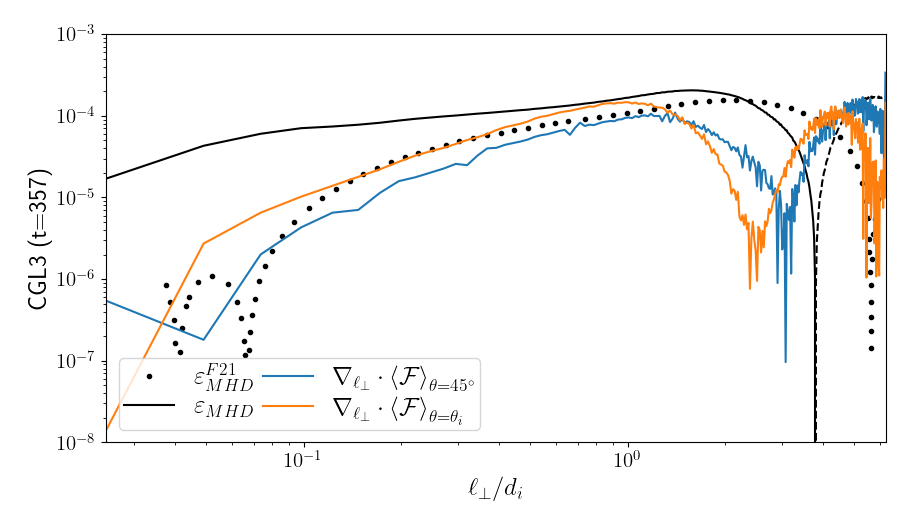
\includegraphics[width=0.9\linewidth,trim=0cm 0cm 0cm 0cm, clip=true]{./Mainmatter/Part_3/images_ch2/CGL3_compa_div}
 \cprotect\caption{Mode de représentation : \cacro{1D} en fonction de \ensuremath{\ell_{\perp}} normalisé par \ensuremath{d_i}. Simu : CGL3 (\ensuremath{t =\num{357}}). Comparaison de \ensuremath{\varepsilon_{MHD}} obtenu par \cacro{F21} (ligne noire pointillée), \cacro{FEL} (ligne noire pleine) et l'application d'une divergence transverse sur \ensuremath{\boldsymbol{\mathcal{F}}} calculés avec \cacro{FEL} et moyenné suivant deux angles \ensuremath{\theta = \ang{45}} de la boîte numérique et \ensuremath{\theta = \theta_i}. }
 \label{fig:compa_div}
 \end{figure} 
 
La \figref{fig:compa_div} illustre les effets de la variation parallèle de la composante parallèle du flux ainsi que ceux du filtrage. Le résultat \cacro{F21} (en pointillé) y est comparé à deux estimations de la divergence transverse effectuée dans nos résultats après avoir moyenné le flux dans le plan perpendiculaire et suivant les $\ell_{\parallel}$. On ne s'attend pas à retrouver exactement le résultat de \cacro{F21} mais à s'en rapprocher. La différence entre les deux estimations correspond au filtrage utilisé dans la moyenne de $\ell_{\parallel}$ : celui utilisé par \cacro{F21} en bleu, et celui que l'on utilise en orange. L'impact de l'angle de filtrage avait déjà été remarqué dans l'analyse de la \figref{fig:rep_CGL1}. On voit ici qu'il a pu influer sur le résultat de \cacro{F21} tout comme il peut influer sur le nôtre. On peut en déduire de cette figure que le poids des variations parallèles, omis par \cacro{F21}, semble avoir un impact sur nos résultats. 
 
 La différence entre nos estimations transverses et \cacro{F21} est située dans le nombre de points du maillage utilisé. Comme \cacro{FEL} prend en compte l'ensemble de l'espace des échelles, il donnera pour $\varepsilon_{MHD}$ par exemple, un résultat impacté par toutes ses variations spatiales omises par une moyenne sur un nombre réduit de vecteurs, malgré la compensation apportée par la pondération. Cet ensemble réduit d'échelles étant choisi tel des multiples de quelques vecteurs directionnels, il représentera d'autant moins les variations en s'approchant des grandes échelles.

 Il semble donc cohérent d'attribuer notre différence de comportement de $\varepsilon_{MHD}$ aux choix numériques façonnant le code de post-traitement. On peut aussi en déduire que \cacro{FEL} donne un résultat associé à la position dans l'espace \sacro{2D} plus réaliste que \cacro{F21}.
 
 \subsection{Effet du forçage sur la zone inertielle} \label{sec-322}
 
 La proximité du forçage induit de fortes variations dans le résultat à grande échelle. De plus, ici, cette injection est loin d'être stationnaire : parfois le forçage est allumé, d'autres fois, il est éteint. Sur la \figref{fig:compainc_t}, est affiché le résultat \cacro{IMHDH} pour différents temps de CGL3. 
 \begin{figure}[!ht]
  \centering
 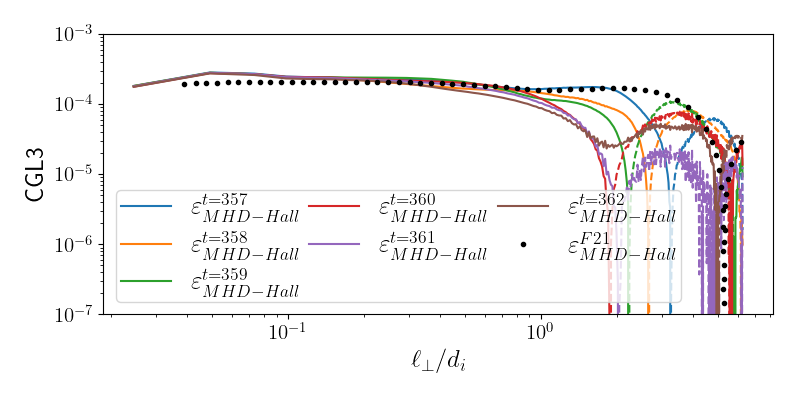
\includegraphics[width=0.9\linewidth,trim=0cm 0cm 0cm 0cm, clip=true]{./Mainmatter/Part_3/images_ch2/F19_time}
 \cprotect\caption{Mode de représentation : \cacro{1D} en fonction de \ensuremath{\ell_{\perp}} normalisé par \ensuremath{d_i}. \ensuremath{\varepsilon_{F19}} est obtenu pour divers temps \ensuremath{t} de CGL3, chaque temps correspond à une couleur. Le résultat extrait de la figure 5 de F21 est donné en pointillés noirs.}
 \label{fig:compainc_t}
 \end{figure} 
 On voit qu'en fonction du temps, l'échelle limite de la zone inertielle (telle que  $\varepsilon_{F19}$ constant) fluctue grandement. Et à $t=357$ (temps utilisé par \cacro{F21}), notre résultat (courbe bleue) montre la zone inertielle la plus large obtenue avec \cacro{FEL}. Le forçage est éteint de $t=357 $ à $t=360$ et la zone inertielle décroît petit à petit.  Puis, pour les temps suivant, il est rallumé et le plateau semble alors se reformer. On observe donc, ici, l'oscillation de l'injection. Aux échelles $\ell_{\perp}/d_i < 1$, le niveau de $\varepsilon_{F19}$ varie peu quel que soit le temps considéré. Cette observation concorde avec l'hypothèse de stationnarité statistique du taux de cascade dans la zone inertielle (ici \cacro{MHDH}). Cette hypothèse est considérée analytiquement pour obtenir des lois du type \cacro{K41} (voir synthèse \ref{synt-01}).  
 
 Le temps de simulation sélectionné impactant l'extension dans la zone de forçage de la zone inertielle, les temps de simulations indiqués dans la \tabref{tab:setups} ont été sélectionnés en prenant garde à l'état allumé ou éteint du forçage, mais cela ne signifie pas que l'extension de la zone inertielle se sera reformée. Une dernière différence, minime, n'a pas encore été abordée : celle de la variation aux petites échelles de $\varepsilon_{MHD-Hall}$. Sa signification associée à l'hyperdissipation sera abordée dans la section \ref{sec-323}.
 
 \section{Équation KHM et incertitude numérique} 
 \label{sec-323}
 
 Afin d'estimer l'incertitude sur nos résultats, nous nous sommes lancés dans la vérification de l'équation \cacro{KHM} du modèle simulé sous sa forme complète et pas seulement de la loi \cacro{K41} dont la validité est réduite à la zone inertielle. Cette estimation est permise par le travail analytique effectué en amont et décrit dans la Partie \ref{part_2}.
 
 \subsection{Calcul de la loi KHM}
 Une loi de type \cacro{KHM} peut s'écrire schématiquement (voir Chapitre \ref{ch-01}) : 
 \begin{equation}
  \label{eq:scheme_KHM_simu}   \partial_t \mathcal{R} =  \varepsilon_{NL} + \varepsilon_{D} + \varepsilon_{F}
 \end{equation}
 Nous avons vu que l'application des hypothèses de Kolmogorov donne la loi réduite de type \cacro{K41} $\varepsilon = - \varepsilon_{NL}$ (voir synthèse \ref{synt-01}). Son contenu, spécifique au modèle implémenté, sera détaillé dans les Chapitres \ref{ch-33} (\sacro{CGLHPe}) et \ref{ch-34} (\sacro{LFHPe}). 
 
 $ \partial_t \mathcal{R}$ est la dérivée temporelle de la fonction de corrélation utilisée pour obtenir la loi exacte. Dans nos études, cette fonction est  $ \mathcal{R} =\frac{1}{4} \left< (\rho'+\rho) (\boldsymbol{v'} \cdot  \boldsymbol{v} +  \boldsymbol{v'_A} \cdot  \boldsymbol{v_A}) + 2\rho' u + 2 \rho u'\right>$. Pour estimer ce terme, on va utiliser les temps consécutifs relevés dans la simulation. La dérivée temporelle sera estimée grâce à des schémas de discrétisation de type \og différences finies \fg{} d'ordre 2 : 
 \begin{itemize}
     \item décentrée vers la droite pour le premier temps $t_0$ : $ (\partial_t \mathcal{R})(t_0) = \frac{\mathcal{R}(t_0 + \delta t) - \mathcal{R}(t_0)}{\delta t}$,
     \item décentrée vers la gauche pour le dernier temps $t_{N_t}$ : $ (\partial_t \mathcal{R})(t_{N_t}) = \frac{\mathcal{R}(t_{N_t}) - \mathcal{R}(t_{N_t}-\delta t)}{\delta t}$,
     \item centrée pour les autres temps :  $ (\partial_t \mathcal{R})(t_n) = \frac{\mathcal{R}(t_{n+1}) - \mathcal{R}(t_{n-1}) }{2\delta t}$ avec $n\in ]0,N_t[$.
 \end{itemize}
 
  Le forçage présent dans nos simulations est un forçage de type antenne de Langevin appliqué sur le champ de vitesse. Par conséquent, le taux de forçage $\varepsilon_{F}$ s'écrira $\varepsilon_{F} = \frac{1}{4} \left< (\rho'+\rho) (\boldsymbol{v'} \cdot  \boldsymbol{f} + \boldsymbol{v} \cdot  \boldsymbol{f'} ) \right>$. Ce forçage dépend de deux composantes aléatoires qui font partie des quantités extraites de la simulation, elles seront notées $f_{sup}$ et $f_{inf}$. Elles permettent de construire une quantité intermédiaire $F = a_1 f_{sup} + (1-a_1) f_{inf}$ avec $a_1$ un paramètre égal à $0.5$ dans nos simulations. Les composantes de $\boldsymbol{f}$ sont alors : $f_x = \partial_y F$, $f_y = - \partial_x F$ et $f_z = 0$. 
  
  Enfin, le taux de dissipation $\varepsilon_{D}$ couvre l'ensemble des hyperdissipations présentes dans le système. Chaque quantité est associée à une hyperdissipation du type $ \nu_X \Delta^4 X$ avec $X$ quantité générique et $\Delta^4 = (\partial^2_x + \partial^2_y + \alpha \partial^2_z)^4$. On va décomposer $\varepsilon_{D}$ tel que : 
  \begin{equation}
      \varepsilon_{D} = \varepsilon^{c}_{D} + \varepsilon^{m}_{D} + \varepsilon^{ui}_{D} + \varepsilon^{ue}_{D}
  \end{equation}
  avec : 
  \begin{itemize}
      \item la contribution cinétique avec $\boldsymbol{D}_{\boldsymbol{v}} = \nu \Delta^4 \boldsymbol{v} $ et $D_{\rho} = \nu_{\rho} \Delta^4 \rho $ :
      \begin{equation}
          \varepsilon^{c}_{D} = \varepsilon^{c}_{D}(\boldsymbol{D_{v}}) + \varepsilon^{c}_{D}(D_{\rho})=   - \frac{1}{4} \left< \left(\rho'+\rho\right) \left(\boldsymbol{v'} \cdot  \boldsymbol{D_{\boldsymbol{v}}} + \boldsymbol{v} \cdot   \boldsymbol{D'_{\boldsymbol{v}}}  \right)\right>   - \frac{1}{4} \left<  \left(D'_{\rho}+D_{\rho}\right)  \boldsymbol{v'} \cdot  \boldsymbol{v}\right> 
      \end{equation}
      \item la contribution magnétique avec $\boldsymbol{D_{v_A}} = \frac{\eta}{\sqrt{\rho}} \Delta^4 (\sqrt{\rho} \boldsymbol{v_A})$ :
      \begin{eqnarray}
          \varepsilon^{m}_{D} = \varepsilon^{m}_{D}(\boldsymbol{D_{v_A}}) + \varepsilon^{m}_{D}(D_{\rho})&=& - \frac{1}{4} \left< \left(\rho'+\rho\right) \left(\boldsymbol{v'_A} \cdot  \boldsymbol{D_{v_A}} + \boldsymbol{v_A} \cdot   \boldsymbol{D'_{v_A}}  \right) \right>\nonumber \\
          &&- \frac{1}{8} \left<\left(\rho'-\rho\right) \left(\frac{D'_{\rho}}{\rho'}-\frac{D_{\rho}}{\rho}\right) \boldsymbol{v'_A} \cdot  \boldsymbol{v_A} \right>
      \end{eqnarray}  
      \item la contribution d'énergie interne ionique (gyrotrope) avec $D_u =  \frac{\nu_p}{2} \Delta^4 (2p_{\perp i } + p_{\parallel i })$ et sachant que $ \rho_i u_i = \frac{1}{2} (2 p_{\perp i } + p_{\parallel i })$:
      \begin{equation}
          \varepsilon^{ui}_{D} = \varepsilon^{ui}_{D}(D_u) + \varepsilon^{ui}_{D}(D_{\rho})=   - \frac{1}{2} \left<  \frac{\rho}{\rho'} D'_u +  \frac{\rho'}{\rho} D_u \right>- \frac{1}{2} \left< \left(\frac{ D'_{\rho}}{\rho'} - \frac{D_{\rho}}{\rho} \right)\left( \rho' u_i  -  \rho u'_i \right)   \right>  
      \end{equation}
      \item la contribution d'énergie interne électronique (isotherme) sachant que  $\rho_e u_e = \rho \ln \rho$ :
      \begin{equation}
          \varepsilon^{ue}_{D} =   - \frac{1}{2} \left<  D'_{\rho} \ln \rho +  D_{\rho} \ln \rho' +  \frac{\rho'}{\rho} D_{\rho} + \frac{\rho}{\rho'} D'_{\rho} \right>  
      \end{equation}
  \end{itemize}
 et $\nu$, $\eta$, $\nu_{\rho}$ et $\nu_p$ des constantes choisies empiriquement pour chaque simulation. Elles sont résumées dans la \tabref{tab:setups_hd}.
 
 %Sachant que dans la majorité des simulations du modèle MCGL, $\nu_{\rho} = 0$ et $\nu_p \ll \nu$, on a négligé les contributions d'énergie interne ainsi que les termes dépendant de $D_{\rho}$ dans les contributions cinétique et magnétique. 
 
 \subsection{Analyse des contributions de la loi KHM }
 
 Sur la \figref{fig:KHM}, $\varepsilon_{NL}$ (bleu) est comparé à un niveau de référence $\varepsilon_{ref} =- \partial_t \mathcal{R}  + \varepsilon_{D} + \varepsilon_{F}$ (violet), construit à partir de $\partial_t \mathcal{R}$ (rouge), $\varepsilon_{D}$ (vert) et $\varepsilon_{F}$ (orange). La différence $\zeta = \varepsilon_{ref} - \varepsilon_{NL}$ est donnée en marron. On remarque qu'elle n'est pas de l'ordre du zéro numérique ($\sim \num{e-20}$) mais environ deux ordres de grandeurs en dessous du niveau de $\varepsilon_{NL}$.  De plus, la forme des termes $\partial_t \mathcal{R}$, $\varepsilon_{D}$ et $\varepsilon_{F}$ est particulière.
 \begin{figure}[!ht]
  \centering
 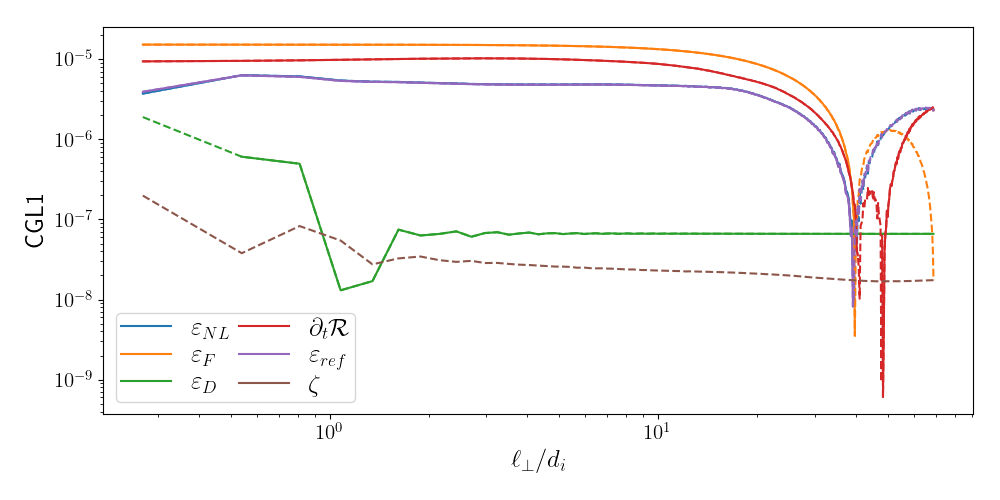
\includegraphics[width=0.9\linewidth,trim=0cm 0cm 0cm 0cm, clip=true]{./Mainmatter/Part_3/images_ch2/CGL1_1D_lperp_alll}
 %\hfill
 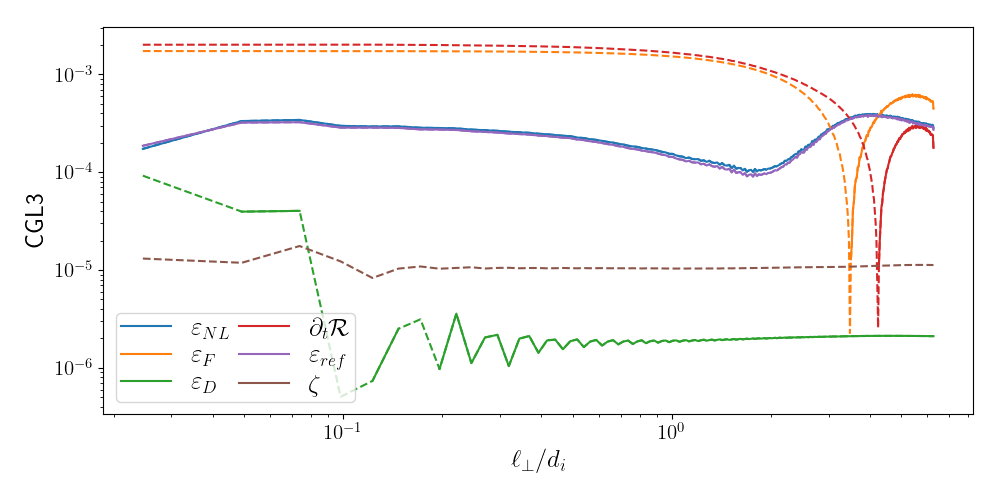
\includegraphics[width=0.9\linewidth,trim=0cm 0cm 0cm 0.5cm, clip=true]{./Mainmatter/Part_3/images_ch2/CGL3_1D_lperp_alll}
 \cprotect\caption{Détail de la loi \cacro{KHM} pour CGL1 (haut) et CGL3 (bas). Bleu : $\varepsilon_{NL}$. Orange : $\varepsilon_{F}$. Vert : $\varepsilon_{D}$. Rouge : $\partial_t \mathcal{R}$. Violet : $\varepsilon_{ref} =- \partial_t \mathcal{R}  + \varepsilon_{D} + \varepsilon_{F}$. Marron : $\zeta = \varepsilon_{ref} - \varepsilon_{NL}$. Représentation : \cacro{1D} en fonction de $\ell_{\perp}$ avec les valeurs positives en trait plein et négatives en trait discontinu. }
 \label{fig:KHM}
 \end{figure} 
 
 \paragraph{Balance des termes et forçage :  } 
 
 Tout d'abord, analysons la situation pour CGL1. Dans le Chapitre \ref{ch-01}, on a vu que : 
 \begin{equation}
     \label{eq:khm_a_verif} \varepsilon_{NL}(\boldsymbol{\ell})  = \varepsilon_{F}(\boldsymbol{\ell}) = \varepsilon_{D}(\boldsymbol{\ell} = 0) = - \varepsilon
 \end{equation}
  dans une zone inertielle où l'hypothèse de stationnarité statistique s'appliquerait. 
  
  On peut en effet identifier une gamme d'échelles $\ell_{\perp}/d_i \in \left[ \num{1}; \num{20}\right]$ telle que $\varepsilon_{NL}$ soit constant. Son niveau est alors d'environ $\num{5e-6}$. La valeur n'est pas visible ici à cause de l'échelle logarithmique mais $\varepsilon_{D}(\boldsymbol{\ell} = 0) \simeq \num{5e-6}$. Donc $\varepsilon_{NL}(\boldsymbol{\ell})  =  \varepsilon_{D}(\boldsymbol{\ell} = 0)$ semble retrouvé. Par contre, même si la constance\footnote{ Le comportement constant du terme de forçage est démontré rigoureusement dans l'annexe \ref{an:forc}.} de $\varepsilon_{F}$ est vérifiée à ces échelles, son niveau est beaucoup trop important, de l'ordre de $ \num{1.5e-5}$. Pour retrouver le niveau $\num{5e-6}$, on doit lui soustraire $\partial_t \mathcal{R}$ qui est d'environ $ \num{1e-5}$. La relation \eqref{eq:khm_a_verif} s'écrit alors dans nos simulations : 
  \begin{equation}
     \label{eq:khm_b_verif} \varepsilon_{NL}(\boldsymbol{\ell})  = \varepsilon_{F}(\boldsymbol{\ell}) - \partial_t \mathcal{R} = \varepsilon_{D}(\boldsymbol{\ell} = 0) = - \varepsilon
 \end{equation}
 
 \paragraph{Analyse du terme \ensuremath{\partial_t \mathcal{R}} :  } 
  Analytiquement, on se servait de l'hypothèse de stationnarité statistique pour annuler $\partial_t \mathcal{R}$, c'est-à-dire pour supposer qu'entre deux temps $\mathcal{R}$ ne varie pas. Puisque $\partial_t \left<E_{tot}\right>=\partial_t \mathcal{R}(\boldsymbol{\ell} = 0)$, si $\partial_t \mathcal{R}=0$ alors $\partial_t \left<E_{tot}\right>=0$.  Sauf que dans nos simulations $\left<E_{tot}\right>$ fluctue légèrement : pour les quatre temps consécutifs utilisés pour CGL1, $\left<E_{tot}\right>$, de l'ordre de $\num{1.3e0}$, augmente d'environ $\num{6e-7}$ par pas de temps. Par conséquent, $\partial_t \mathcal{R}=0$ est impossible à obtenir. C'est ce que l'on observe sur la \figref{fig:KHM} pour CGL1 comme pour CGL3. Pourtant, la convergence temporelle des résultats du calcul de loi exacte \cacro{K41} dans une certaine zone d'échelles a bel et bien été observée sur la \figref{fig:compainc_t}, et cela nous semblait une belle preuve de la stationnarité statistique de nos simulations. À première vue, ces résultats ne semblent pas compatibles. L'interprétation de ce paradoxe reste à affiner mais le comportement du $\partial_t \mathcal{R}$ instantané tel un forçage ne semble pas être une spécificité de nos simulations. En effet, \cite{ferrand_-depth_2022} trouvent un comportement similaire dans des simulations de turbulence non forcée, pour lesquelles l'énergie totale moyenne est en  décroissance perpétuelle. Dans notre cas, on pourrait peut-être interpréter le comportement du terme $\partial_t \mathcal{R}$ comme un réservoir d'énergie régulant temporellement l'injection de l'énergie dans la cascade afin que cette dernière puisse s'effectuer au taux imposé par les processus de dissipation. 
 
  \paragraph{Analyse des contributions d'hyperdissipation :  } 
  
   Un autre comportement pathologique est celui de $\varepsilon_{D}$ en fonction de $\ell$. Dans la théorie analytique, ce terme est supposé nul à toutes les échelles sauf en $\ell = 0$ à cause de l'anomalie dissipative. Dans nos simulations, son rôle est joué par les termes d'hyperdissipation, mais on s'attendrait à ce qu'ils décroissent rapidement en allant vers les grandes échelles puisque la dérivation par $\Delta^4$ impose un comportement en $k^8$ dans l'espace de Fourier. Regardons ce qu'il en est en le décomposant sur ses diverses contributions. La décomposition est présentée sur la \figref{fig:DISS}. 
 \begin{figure}[!ht]
  \centering
 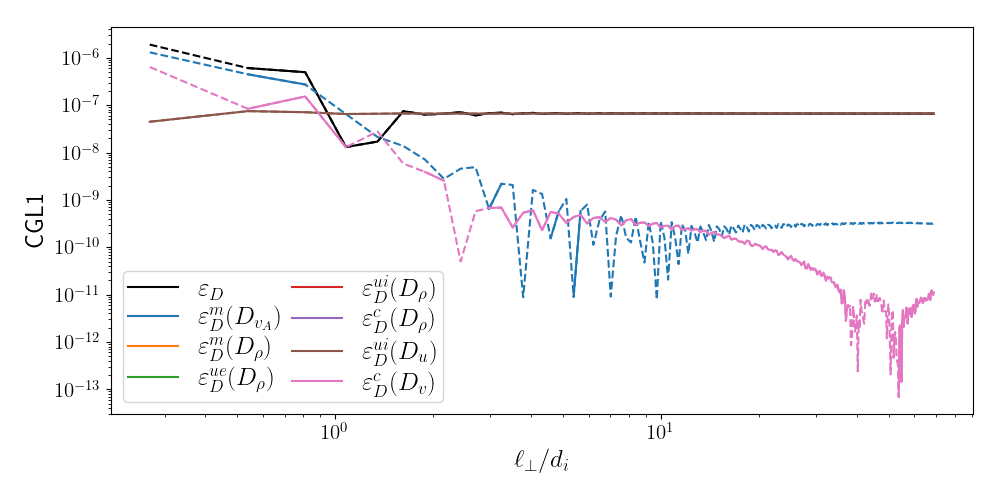
\includegraphics[width=0.9\linewidth,trim=0cm 0cm 0cm 0cm, clip=true]{./Mainmatter/Part_3/images_ch2/CGL1_1D_lperp_dissl}
 %\hfill
 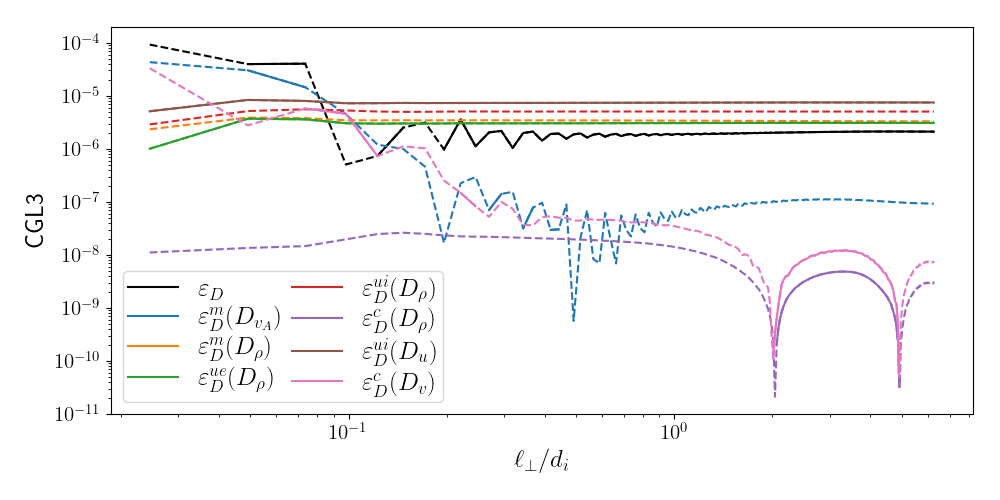
\includegraphics[width=0.9\linewidth,trim=0cm 0cm 0cm 0.5cm, clip=true]{./Mainmatter/Part_3/images_ch2/CGL3_1D_lperp_dissl}
 \cprotect\caption{Détail du terme d'hyperdissipation, $\varepsilon_{D}$ (noir), pour CGL1 (haut) et CGL3 (bas). Bleu : $\varepsilon^m_{D}(D_{\boldsymbol{v_A}})$. Orange :  $\varepsilon^m_{D}(D_{\rho})$. Vert :  $\varepsilon^{ue}_{D}(D_{\rho})$. Rouge : $\varepsilon^{ui}_{D}(D_{\rho})$. Violet :  $\varepsilon^c_{D}(D_{\rho})$ Marron :  $\varepsilon^{ui}_{D}(D_{u})$. Rose :  $\varepsilon^c_{D}(D_{v})$. Représentation : \cacro{1D} en fonction de $\ell_{\perp}$ avec les valeurs positives en trait plein et négatives en trait discontinu.}
 \label{fig:DISS}
 \end{figure}
 On y voit que chacune des contributions semble ou décroître en allant vers les grandes échelles ou rester constante. Les termes en $D_{\rho}$ (visibles seulement pour CGL3 puisque $\nu_{\rho} = 0$ pour CGL1) et $D_u$ ne montrent pas de décroissance, et la tendance en environ $\ell^{-2}$ de la décroissance de $\varepsilon^{c}_{D}(\boldsymbol{D_{v}})$ et $\varepsilon^{m}_{D}(\boldsymbol{D_{v_A}})$ avait été remarquée par \cite{ferrand_multi-scale_2021} dans le cas incompressible. La pathologie de cette pente en $-2$ y avait été identifiée et associée à une saturation mathématique de la fonction de corrélation calculée entre deux points. Cette saturation est due à une puissance de $k$ trop importante dans l'espace de Fourier et est similaire à celle relevée par \cite{cho_simulations_2009}. 
 
 Dans l'Annexe \ref{an:sat}, nous proposons une démonstration mathématique de ce phénomène en fonction du type de la fonction de corrélation, incrémentale ou non, et de la tendance du spectre dans l'espace de Fourier. On y obtient dans le cas non incrémental, pour la corrélation de deux quantités indéfinies $A$ et $B$, : 
 \begin{eqnarray}
   \label{eq:sat_noninc}  \left<A({\bf x} + \boldsymbol{\ell})  \cdot B({\bf x}) + A({\bf x})  \cdot B({\bf x} + \boldsymbol{\ell})\right> 
 \propto \left\{
     \begin{aligned}
     &\ell^{-2}& \textrm{si $m \in ]-\infty,-1[$ } \\
  &\ell^{m-1}&  \textrm{si $m \in ]-1,1[$}  \\
  &1& \textrm{si $m \in ]1,+\infty[$ } 
 \end{aligned}
 \right.%\nonumber  \\
 \end{eqnarray}
 avec $m$, la pente du spectre unidimensionnel en représentation logarithmique tel que $k^{-m}$. 
 
 Pour une fonction de corrélation incrémentale on obtient :
 \begin{eqnarray}
    \label{eq:sat_inc} \left<(A({\bf x} + \boldsymbol{\ell}) - A({\bf x}))\cdot(B({\bf x} + \boldsymbol{\ell}) - B({\bf x})) \right> 
 \propto \left\{
     \begin{aligned}
     & 1 & \textrm{si $m \in ]-\infty,1[$ } \\
 & \ell^{m-1}&  \textrm{si $m \in ]1,3[$ }  \\
 & \ell^2 & \textrm{si $m \in ]3,+\infty[$}
 \end{aligned}
 \right. .%\nonumber\\
 \end{eqnarray}
 Si l'on analyse les différentes contributions du terme de dissipation, on se rend compte que $ \varepsilon^{c}_{D}(\boldsymbol{D_{v}}) $, $ \varepsilon^{c}_{D}(D_{\rho})$, $\varepsilon^{m}_{D}(\boldsymbol{D_{v_A}}) $,
 $ \varepsilon^{ui}_{D}(D_u) $ et $\varepsilon^{ue}_{D}$ ont une forme assez proche d'une fonction de corrélation non incrémentale et $ \varepsilon^{m}_{D}(D_{\rho}) $ tandis que  $\varepsilon^{ui}_{D}(D_{\rho})$ sont plus proches d'une fonction incrémentale. 
 
 Pour une pente de spectre autour de $k^8$ ($m=-8$), une fonction de corrélation non incrémentale va saturer en $\ell^{-2}$. On retrouve ce comportement pour $ \varepsilon^{c}_{D}(\boldsymbol{D_{v}}) $ et  $\varepsilon^{m}_{D}(\boldsymbol{D_{v_A}}) $. Tandis qu'une fonction de corrélation incrémentale va saturer en $\ell^0$ (comportement retrouvé pour  $ \varepsilon^{m}_{D}(D_{\rho}) $ et  $\varepsilon^{ui}_{D}(D_{\rho})$). On retrouve aussi le comportement du terme de forçage (fonction de corrélation non incrémentale) constant loin des échelles de forçage, puisqu'un Dirac à petit $\ell$ peut-être vu comme une pente en $m = +\infty$. Ces comportements plus mathématiques que physiques sont retrouvés pour toutes les simulations. 
 
 On remarque tout de même les fortes variations des termes décroissant en $\ell^{-2}$. Ces variations sont la cause de la bosse visible aux plus petites échelles pour tous les taux $\varepsilon_{NL}$ et $\varepsilon$ calculés dans les simulations et que l'on avait remarquée dans la section \ref{sec-321}. En effet, $\varepsilon_F - \partial_t \mathcal{R} $ reste constant dans cette zone alors que la bosse apparaît dans $\varepsilon_F - \partial_t \mathcal{R} + \varepsilon_D $. Cette bosse nous indique donc les échelles auxquelles l'erreur mathématique de l'hyperdissipation impacte systématiquement $\varepsilon_{NL}$ et ses contributions.  
 
  Ce type d'erreur mathématique pourrait aussi impacter $\partial_t \mathcal{R}$, $\mathcal{R}$ étant une fonction de corrélation en deux points.
  
  \subsection{Estimation de l'erreur sur le taux de cascade  } 
 
 Les fonctions de corrélation en deux points ne sont donc pas adaptées à l'étude de la physique des termes d'hyperdissipation et de ceux inclus dans $\partial_t \mathcal{R}$ comme a pu le faire remarquer \cite{cho_simulations_2009}\footnote{La solution proposée par \cite{cho_simulations_2009} est d'augmenter le nombre de points servant au calcul de la fonction de corrélation. Une telle tâche s'annonce mathématiquement complexe et lourde dans le cadre de la théorie des lois exactes. Une autre possibilité est d'estimer précisément pour chaque contribution la puissance $m$ du spectre influant sur le résultat de chaque contribution au taux de dissipation, puis de calculer la tendance attendue en $\ell^{m-1}$ [\cite{ferrand_multi-scale_2021}].}. Par la suite, nous nous concentrerons seulement sur $\varepsilon_{NL}$ et ses contributions, mais nous garderons en mémoire les influences potentielles de ces termes.
 
 L'analyse des différentes contributions à la loi \cacro{KHM} permet ainsi d'identifier les sources d'erreurs numériques et mathématiques menant au niveau de $\zeta$. Ce dernier, de l'ordre des fluctuations de $\left< E_{tot}\right>$, reflèterait la signature de la quasi-stationnarité statistique des simulations. Aux échelles plus faibles, la saturation mathématique du calcul des fonctions de corrélation dépendant de l'hyperdissipation ainsi que sa signature\footnote{Les corrélations impliquées dans $\varepsilon_{D}$ étant d'ordre 2 et celles présentes dans les termes dominant de $\varepsilon_{NL}$ étant d'ordre 3, le reflet dans $\varepsilon_{NL}$ de l'erreur mathématique pourrait, à priori, ne pas compenser exactement l'erreur sur $\varepsilon_{D}$. } dans $\varepsilon_{NL}$ semblent impacter $\zeta$. Ce dernier correspond donc à l'incertitude systématique de notre estimation du taux de cascade, incertitude provenant des données initiales, de leur adéquation avec les hypothèses de Kolmogorov et du schéma numérique utilisé pour le calcul des termes des lois exactes. Par la suite, les contributions qui apparaîtront inférieures à $\zeta$ seront alors supposés dans la zone d'incertitude du taux de cascade total. Leur analyse devra donc être effectuée avec précautions. 
 
 Un autre point reste à éclaircir dans cette étude sur les lois du type \cacro{KHM} : la différence entre la loi obtenue en utilisant $\mathcal{R}$ et celle en utilisant une fonction incrémentale $\mathcal{S}$. La fonction $\mathcal{S}$ associée à $\mathcal{R}$ est :
 \begin{equation}
    \label{eq:scheme_khms} \mathcal{S} = \frac{1}{4} \left< \delta (\rho \boldsymbol{v}) \cdot \delta \boldsymbol{v} + \delta (\rho \boldsymbol{v_A}) \cdot \delta \boldsymbol{v_A}  + 2 \delta \rho \delta u \right>
 \end{equation}
 On a alors la relation $\mathcal{S} = \left<E_{tot}\right> - \mathcal{R}$. Sachant que $\mathcal{R}(\boldsymbol{\ell} = 0) = \left<E_{tot}\right>$, il est facile de passer de l'expression \eqref{eq:scheme_KHM_simu} à la loi :
 \begin{equation}
  \label{eq:scheme_KHMS_simu}   \partial_t \mathcal{S} = - \mathcal{E}_{NL} + \mathcal{E}_{D} + \mathcal{E}_{F}
 \end{equation}
 avec $\mathcal{E}_{NL} = \varepsilon_{NL}(\boldsymbol{\ell} = 0) - \varepsilon_{NL}$, $\mathcal{E}_{D} = \varepsilon_{D}(\boldsymbol{\ell} = 0) - \varepsilon_{D}$ et $\mathcal{E}_{F} = \varepsilon_{F}(\boldsymbol{\ell} = 0) - \varepsilon_{F}$. 
 
 \begin{figure}[!ht]
  \centering
 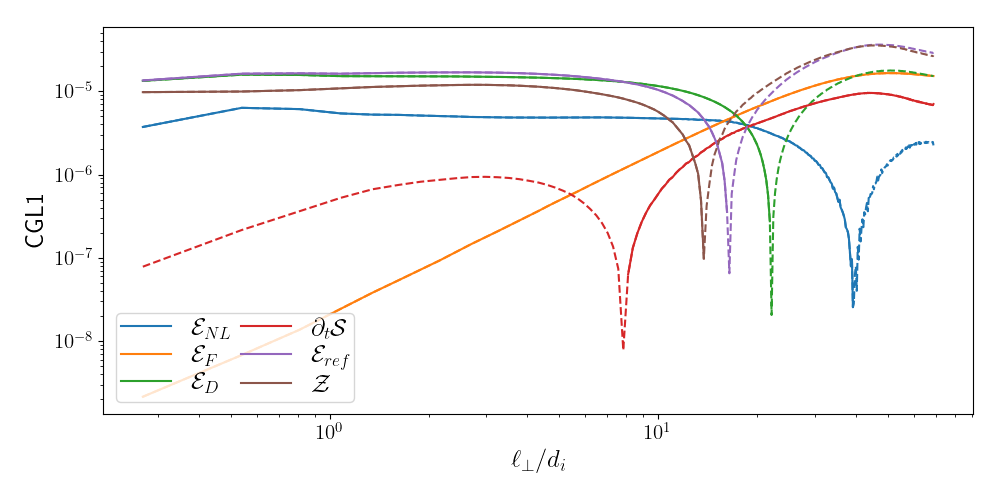
\includegraphics[width=0.9\linewidth,trim=0cm 0cm 0cm 0cm, clip=true]{./Mainmatter/Part_3/images_ch2/CGL1_1D_lperp_allSl}
 %\hfill
 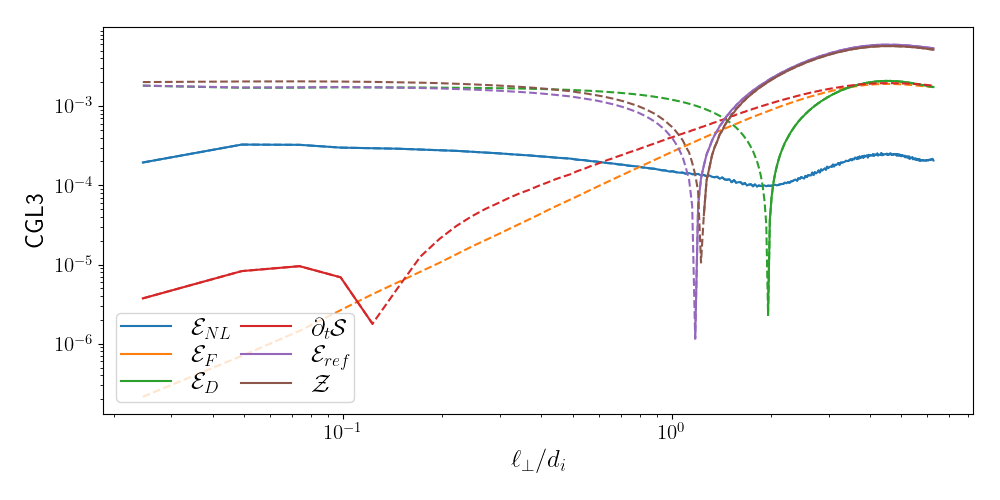
\includegraphics[width=0.9\linewidth,trim=0cm 0cm 0cm 0.5cm, clip=true]{./Mainmatter/Part_3/images_ch2/CGL3_1D_lperp_allSl}
 \cprotect\caption{Détail de la loi \eqref{eq:scheme_khms} pour CGL1 (haut) et CGL3 (bas). Bleu : \ensuremath{\mathcal{E}_{NL}}. Orange : \ensuremath{\mathcal{E}_{F}}. Vert : \ensuremath{\mathcal{E}_{D}}. Rouge : \ensuremath{\partial_t \mathcal{S}}. Violet : \ensuremath{\mathcal{E}_{ref} =- \partial_t \mathcal{S}  + \mathcal{E}_{D} + \mathcal{E}_{F}}. Marron : \ensuremath{\mathcal{Z} = \mathcal{E}_{ref} - \mathcal{E}_{NL}}. Représentation : \cacro{1D} en fonction de \ensuremath{\ell_{\perp}} avec les valeurs positives en ligne pleine et négatives en ligne dicontinue. }
 \label{fig:KHMS}
 \end{figure}
 
On notera que l'équation d'énergie totale s'écrit sous la forme $\partial_t E_{tot} + \nabla \cdot \boldsymbol{F_{tot}} = S$ avec $S$ les termes sources (dissipation et forçage), et $\boldsymbol{F_{tot}}$ le total de flux. De plus, puisque $\left<  \nabla \cdot \boldsymbol{F_{tot}} \right> = \nabla_{\boldsymbol{\ell}} \cdot \left< \boldsymbol{F_{tot}} \right> = - \left<  \nabla' \cdot \boldsymbol{F_{tot}} \right> = 0$, alors $\mathcal{E}_{NL} =  - \varepsilon_{NL}$.
 
 
 En appliquant cette transformation sur le détail de la loi \cacro{KHM} (\figref{fig:KHM}), on obtient les résultats de la  \figref{fig:KHMS}. On y remarque que le comportement des termes de forçage (orange) et de dissipation (vert) se sont inversés. $\mathcal{E}_{F}$ augmente en allant des petites vers les grandes échelles, avec une pente de facteur $2$, et $\mathcal{E}_{D} $ reste constant avant de changer de signe vers les grandes échelles. Ces comportements sont cohérents avec ceux démontrés dans les Annexes \ref{an:forc} et \ref{an:sat} (voir équations \eqref{eq:sat_noninc} et \eqref{eq:sat_inc}). Par contre, la différence $ \mathcal{Z} = \mathcal{E}_{ref} - \mathcal{E}_{NL} = (- \partial_t \mathcal{S} + \mathcal{E}_{D} + \mathcal{E}_{F}) - \mathcal{E}_{NL}$ est supérieure à $\zeta$. L'utilisation d'une fonction de corrélation incrémentale dans une étude de données de simulations semble donc amplifier l'erreur numérique et mathématique associée aux termes temporels, de dissipation et de forçage en y ajoutant l'erreur sur l'équation de $\left<E_{tot}\right>$. 
 
 %\newpage
 \section{Synthèse des tests de validation et sources d'erreurs }
 \label{synt-32}
 \fcolorbox{red}{white}{\begin{minipage}[c]{\linewidth}
 Ces études sont illustrées par les résultats obtenus pour les simulations CGL1 et CGL3. 
 
 \paragraph{Comparaison Inc-MHD-Hall avec les résultats de \cite{ferrand_multi-scale_2021} :}
 \begin{itemize}
     \item le comportement des lois \cacro{IMHDH} est retrouvé,
     \item effets de nos choix de schéma numérique. 
 \end{itemize}
 
 \paragraph{Effet du forçage sur la zone inertielle visualisée avec Inc-MHD-Hall :}
 \begin{itemize}
     \item visualisation des oscillations induites par l'injection d'energie dans le taux de cascade : extension/réduction de la zone inertielle sur environ une demi décade,
     \item visualisation de l'impact de la stationnarité statistique : amortissement des oscillations et convergence de la zone inertielle.
 \end{itemize}
 
 % \paragraph{Comparaison MHD incompressible avec la formulation de PP98 donnée par \cite{banerjee_alternative_2017} : }
 % \begin{itemize}
 %     \item comportement global retrouvé
 %     \item  différences induites par la quasi-incompressibilité des simulations
 % \end{itemize}
 
 % \paragraph{Comparaison MHD compressible avec pression isotrope avec les prédictions de \cite{andres_energy_2018} : }
 % \begin{itemize}
 %     \item  formulation f1 cohérente avec les prédictions
 %     \item validation de l'apport de f2 sur f1 et cohérence avec les prédictions
 % \end{itemize}
 
 \paragraph{Analyse de la loi KHM : }
 \begin{itemize}
     \item paradoxe sur l'hypothèse de stationnarité statistique dans les simulations,
     \item saturation mathématique apportée par l'hyperdissipation,
     \item incertitude provenant de l'utilisation de fonctions incrémentales,
     \item estimation de l'erreur numérique et mathématique sur la loi exacte totale associée au modèle simulé, noté $\zeta$. \\
 \end{itemize}
 
 {\bf Ces études valident le schéma numérique et son implémentation, et questionnent les comportements non-physiques pouvant impacter les résultats.} \\
 
 Les Annexes \ref{an:A} et \ref{an:B} contiennent des études complémentaires pour ce chapitre.
 \end{minipage}}
